\section{Kompilierung und Programmierung}\label{section:konzeption:kompilierung-und-programmierung}

% \begin{note}
%     \textbf{Notizen:}
%     \begin{itemize}
%         \item Erwähnung von \autoref{requirement:Kompilierung} und \autoref{requirement:Programmierung von Steuereinheiten}
%         \item Beschreibung der CrossLab-Services + Klassendiagramme
%         \item Konzept für die Bereitstellung von Compilern als Laborgeräte
%         \item Beschreibung der Einbindung in die betrachtete Experimentkonfiguration
%         \item (Beschreibung möglicher Einstellungen?)
%     \end{itemize}
% \end{note}

Nach \autoref{requirement:Kompilierung} soll die Kompilierung der Programme von Nutzern innerhalb der IDE ermöglicht werden. Laut Unteranforderung (a) soll daher ein CrossLab-Service für die Bereitstellung und Nutzung von Compilern entwickelt werden. Diese sollen nach Unteranforderung (b) von der IDE für die Nutzung von Compilern verwendet werden. Weiterhin soll nach \autoref{requirement:Programmierung von Steuereinheiten} die Programmierung von Steuereinheiten innerhalb der IDE ermöglicht werden. Laut Unteranforderung (a) soll daher ein CrossLab-Service für die Programmierung von Steuereinheiten entwickelt werden. Dieser soll nach Unteranforderung (b) von der IDE für die Programmierung von Steuereinheiten verwendet werden. Dementsprechend werden im Folgenden der \textit{Compilation Service} sowie der \textit{Programming Service} vorgestellt.

In \autoref{figure:klassendiagramm-compilation-service} ist ein Klassendiagramm für den Compilation Service angegeben. Dabei besitzt der Compilation Service Consumer nur eine Funktion \texttt{compile()}, die es ermöglicht, die Kompilierung eines Ordners anzufragen. Dabei können zusätzliche Optionen für den Compiler sowie das gewünschte Format der Ausgabe angegeben werden. Die möglichen Ausgabeformate können auf der Seite des Compilation Service Producer über entsprechende Schemata definiert und über die Funktion \texttt{addResultFormat()} hinzugefügt werden. Die registrierten Ausgabeformate können dann in der Servicebeschreibung des Compilation Service Producer hinterlegt werden. Während der Erstellung eines Experiments kann das gewünschte Ausgabeformat für die Verbindung eines Compilation Service Consumer und eines Compilation Service Producer in der Verbindungskonfiguration angegeben werden. Die Behandlung eingehender Kompilieranfragen kann durch Event Handler für \texttt{Compile}-Events des Compilation Service Producer erfolgen. Die Behandlung von Kompilieranfragen ist abhängig vom verwendeten Compiler. Bei einer erfolgreichen Kompilierung wird das Ergebnis in dem festgelegten Ausgabeformat zusammen mit den Meldungen des Compilers an den Compilation Service Consumer gesendet. Falls die Kompilierung fehlschlägt, werden nur die Fehlermeldungen des Compilers versendet.

\begin{figure}[tbp]
    \centering
    \begin{tikzpicture}
        \begin{class}[text width=6.5cm]{CompilationServiceProducer}{0,0}
            \operation{+ addResultFormat()}
            \operation{+ onCompile()}
        \end{class}
        \begin{class}[text width=6.5cm]{CompilationServiceConsumer}{7.5,0}
            \operation{+ compile()}
        \end{class}
    \end{tikzpicture}
    \caption{Klassendiagramm Compilation Service}
    \label{figure:klassendiagramm-compilation-service}
\end{figure}

\begin{figure}[tbp]
    \centering
    \begin{tikzpicture}
        \begin{class}[text width=6.5cm]{ProgrammingServiceProducer}{0,0}
            \operation{+ onProgram()}
        \end{class}
        \begin{class}[text width=6.5cm]{ProgrammingServiceConsumer}{7.5,0}
            \operation{+ program()}
        \end{class}
    \end{tikzpicture}
    \caption{Klassendiagramm Programming Service}
    \label{figure:klassendiagramm-programming-service}
\end{figure}

In \autoref{figure:klassendiagramm-programming-service} ist ein Klassendiagramm für den Programming Service angegeben. Dabei besitzt der Programming Service Consumer nur die Funktion \texttt{program()}, die es ermöglicht, eine Programmieranfrage zu starten. Diese muss entweder eine Datei, z.B. das Ergebnis einer Kompilierung, oder einen Ordner mit dem entsprechenden Programm enthalten. Dabei könnte der Programming Service Producer über seine Servicebeschreibung angeben, welche Formate unterstützt werden. Der Programming Service Producer löst bei einer eingehenden Programmieranfrage ein entsprechendes \texttt{Program}-Event aus. Dieses kann durch entsprechende Event Handler abgefangen und zur Programmierung der Steuereinheit verwendet werden.

Die betrachtete Experimentkonfiguration wird zunächst um ein weiteres Laborgerät erweitert. Dieses stellt einen Compiler über einen entsprechenden Compilation Service Producer bereit. Die IDE wird um einen Compilation Service Consumer sowie einen Programming Service Consumer erweitert. Die Steuereinheit wird um einen Programming Service Producer erweitert. Die IDE wird dann über die neu hinzugefügten CrossLab-Services mit dem Compiler und der Steuereinheit verbunden.

\begin{figure}[htbp]
    \centering
    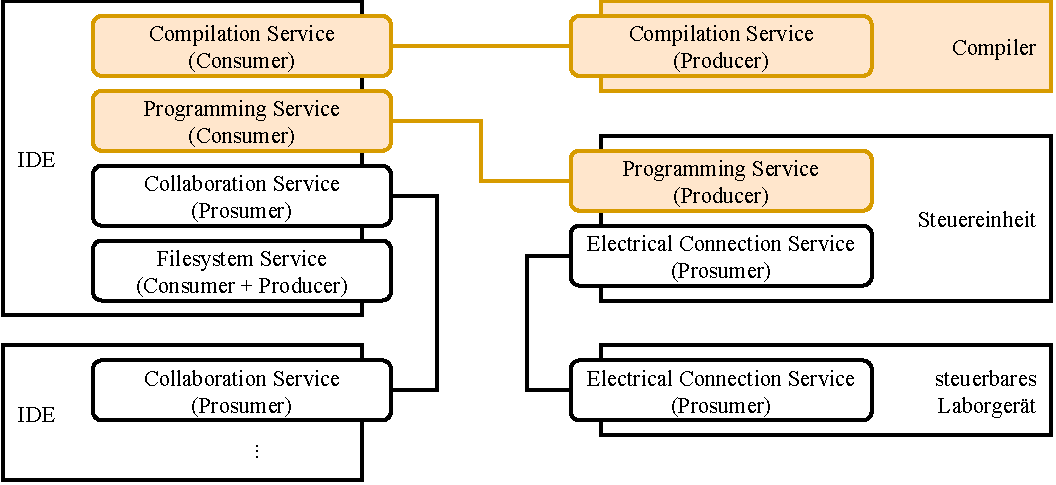
\includegraphics[width=\textwidth]{diagrams/experimentkonfigurationen/Experimentkonfiguration-03.drawio.pdf}
    \caption{Experimentkonfiguration}
    \label{figure:experimentkonfiguration:kompilierung}
\end{figure}